%%%%%%%%%%%%%%%%%%%%%%%%%%%%%%%%%%%%%%%%%%%%%%%%%%%%%%%%%%%%%%%%%%%%%%%%%%
 %																		%
 %	Plantilla Latex para presentación del proyecto de curso				%
 %	Programación de Aplicaciones para Internet y la Nube					%
 %																		%
 %	Creada por: Duván Pardo, Wilson López								%
 %																		%
 %	Versión: 0.1															%
 %	Dapardoc@gmail.com ; Wilrilo@gmail.com								%
 %																		% 
 %	Se requieren los archivos plantilla.bbl y							% 
 %	El directorio Imagenes que contiene: CECAD,DC, Elementos y RITA		%  
 %																		%
%%%%%%%%%%%%%%%%%%%%%%%%%%%%%%%%%%%%%%%%%%%%%%%%%%%%%%%%%%%%%%%%%%%%%%%%%%

\documentclass[10pt]{article}   			% Describe el tipo de documento, y el tamaño de la letra del texto

\usepackage[utf8]{inputenc}				% Define codificación para que permita caracteres latinos (acentos)
\usepackage[spanish,activeacute]{babel} 	% Paquete para poder escribir con tildes y otros caracteres especiales

\usepackage{vmargin}						% Código para margenes y formato de página
\setpapersize{A4}
\setmargins	{2.2cm}     					% margen izquierdo
			{1 cm}                 		% margen superior
			{16.5cm}               		% anchura del texto
			{23.42cm}             		% altura del texto
			{20pt}                		% altura de los encabezados
			{1.2cm}               		% espacio entre el texto y los encabezados
			{0pt}                		% altura del pie de página
			{2cm}                 		% espacio entre el texto y el pie de página

\usepackage{amsmath}						% paquete para expresiones matemáticas
\usepackage{amsfonts}					% paquete para escritura de ecuaciones 
\usepackage{amssymb}						% paquete para caracteres especiales para ecuaciones 

\usepackage{fancyhdr}					% Temas para encabezado y pie de pagina
\usepackage{fancyvrb}
\pagestyle{fancy} 
\usepackage{float}
\pagenumbering{arabic} 					% Numeración de paginas {arabic roman}
\usepackage{hyperref}					% Para hipervinculos
\usepackage{graphicx}					% Para incluir imágenes
\usepackage{caption}						% Descripciones de las figuras
\usepackage{subcaption}					% Descripción varias imagenes en usa sola figura
\graphicspath{ {Imagenes/} }				% Directorio de imágenes esta capeta va donde esta el archivo tex


\usepackage{color, colortbl}				% Colores para tablas
\usepackage{listings}					% Para el código Fuente
\usepackage{xcolor}						% para color en codigos o listrings
\definecolor{limegreen}{RGB}{50,100,50}	% Definición de colores ejemplo verde en RGB
\definecolor{Red}{RGB}{220,120,120}		% se definen colores para la tabla en el cronograma pueden ser RGB 0-255 o rgb 0-1 cada componente
\definecolor{LightCyan}{rgb}{0.88,1,1}
\definecolor{azul}{RGB}{120,120,210}

\lstset{numbers=left, numberstyle=\tiny, stepnumber=2, numbersep=5pt}

%Aquí inicia el documento.
\begin{document}
	% Se define el Encabezado
	%clhead[]{Proyecto}
	\lhead[]{Programación de Aplicaciones para Internet y la Nube}
	\rhead[]{\textbf{2016-I}}
	\renewcommand{\headrulewidth}{0.5pt}

	\thispagestyle{empty}						% La primera página no lleva estilo (sin encabezado)
	\begin{center}
		\large {Programación de Aplicaciones para Internet y la Nube
			\hspace{5 cm}\textbf{2016-I}}
		\bigskip  
		\textbf{
				\LARGE{\\TALLER 2}}\\								% Nombre del proyecto
	\end{center}	
	\begin{flushright}	
		\bigskip	
		Nombre del Estudiante: \textbf{Duván Pardo, Wilson López}			% Nombre del estudiante
	\end{flushright} 

\section{INTRODUCCIÓN}	
Cientos de las marcas más grandes del mundo confían en OpenStack para manejar sus negocios todos los días, lo que reduce los costes y ayudar a que se muevan más rápido. OpenStack tiene un fuerte ecosistema, y los usuarios que buscan apoyo comercial puede elegir entre diferentes productos y servicios OpenStack-powered en el mercado. El software está construido por una próspera comunidad de desarrolladores, en colaboración con los usuarios, y está diseñado para solventar nuestras necesidades.\\


Para cumplir con estos principios OpenStack está divido en diferentes componentes que trabajan en conjunto. Esta integración es lograda a través de interfaces de programación de aplicaciones – APIs – que cada servicio ofrece y consume, gracias a estas APIs, los servicios pueden comunicarse entre ellos y además se posibilita que un servicio sea reemplazado por otro de similares características siempre que se respete la forma de comunicación. Es decir, OpenStack es extensible y se ajusta a las necesidades de quien desee implementarlo.( tomado de \href{http://vmartinezdelacruz.com/en-pocas-palabras-como-funciona-openstack/}{¿Cómo funciona OpenStack?} y \href{https://www.openstack.org/}{openstack})\\

\textbf{OpenStack y RedHat:}“Las personas tienden a optar por las mejores ideas. En 2004, Linux® se parecía mucho al actual OpenStack®. OpenStack está creciendo rápidamente, con el apoyo de una comunidad de individuos y empresas, y creando una plataforma que todos podemos usar para crear nubes abiertas enormemente escalables. Por eso creemos que OpenStack es el mejor exponente de la tecnología de nube.” (tomado de \href{https://www.redhat.com/es/insights/openstack}{RedHat})








	
\section{OBJETIVO}
Realizar despliegues de infraestructura utilizando el lenguaje de orquestación de OpenStack. En particular, realizar un despliegue multi-instancia cuyos servicios deben colaborar.
\section{ACTIVIDADES}	

\textbf{Antes de comenzar con el taller es es necesaria la instalación de algunos elementos antes de iniciar, se resume en el siguiente código para ubuntu 14.04 lts}
\begin{small}
	\begin{lstlisting}[frame=single]	
	sudo apt-get -y install python-pip python-dev
	sudo pip2 install virtualenv
	nano creds
	export OS_TENANT_ID=0689b2eb69a24f5eafccdbd88a20c8a7
	export OS_TENANT_NAME=cloud1
	export OS_PROJECT_NAME=cloud1
	export OS_USERNAME=grupo1
	export OS_PASSWORD=1grupo
	export OS_AUTH_URL="http://10.20.230.15:5000/v2.0"
	export OS_REGION_NAME=regionOne
	source creds
	virtualenv venv
	source venv/bin/activate
	(venv) $ pip install python-heatclient
	(venv) $ openstack stack list	
	\end{lstlisting}
\end{small}
\newpage
A continuación se observa el la ejecución en consola.\\


\begin{figure}[ht]
	\centering
	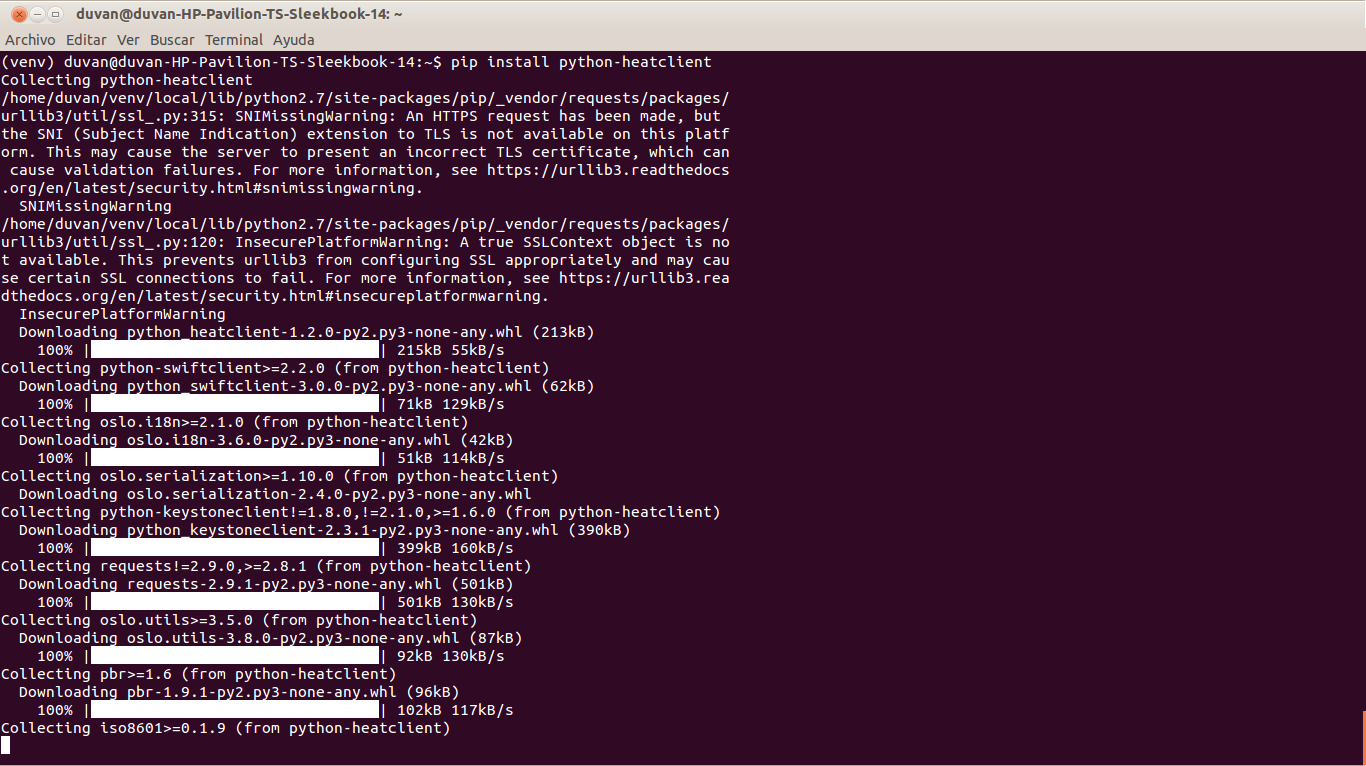
\includegraphics[scale=0.28]{heat}  
	\caption{Preparación del entorno} \label{fig:Elementos}
\end{figure}

\begin{figure}[ht]
	\centering
	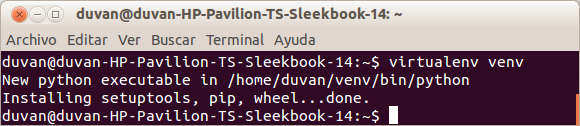
\includegraphics[scale=0.6]{venv}  
	\caption{Preparación del entorno} \label{fig:Elementos}
\end{figure}

 \begin{enumerate}
	\item Crear un directorio “\texttt{\href{https://github.com/wilrilo/talleres/tree/master/file/taller2/wordpress-heat}{wordpress-openstack}}”, y dentro de ese directorio, un sub-directorio “\texttt{lib}”. \\
	
	
	\begin{figure}[ht]
		\centering
		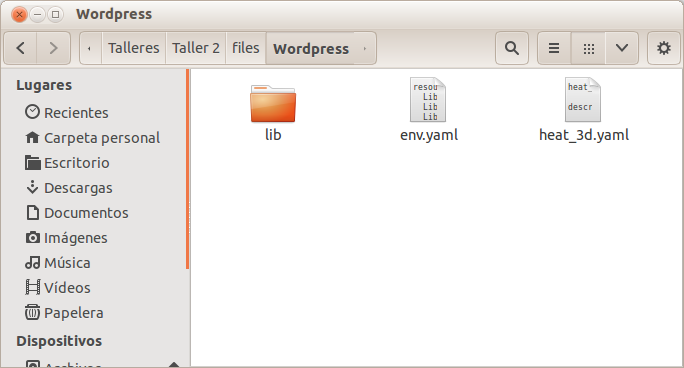
\includegraphics[scale=0.3]{Folder1}  
		\caption{Directorio creado}
	\end{figure}
	


	\item 	Descargar los archivos   
	\href{https://raw.githubusercontent.com/miguelgrinberg/heat-tutorial/master/lib/mysql.yaml}{mysql.yaml} ,
	\href{https://raw.githubusercontent.com/miguelgrinberg/heat-tutorial/master/lib/wordpress.yaml}{wordpress.yaml},
	\href{https://raw.githubusercontent.com/miguelgrinberg/heat-tutorial/master/lib/private\_network.yaml}{private\_network.yaml} y
	\href{https://raw.githubusercontent.com/miguelgrinberg/heat-tutorial/master/lib/floating\_ip.yaml}{floating\_ip.yaml} en el directorio “\texttt{lib}”. \\
	
	

\begin{figure}[ht]
	\centering
	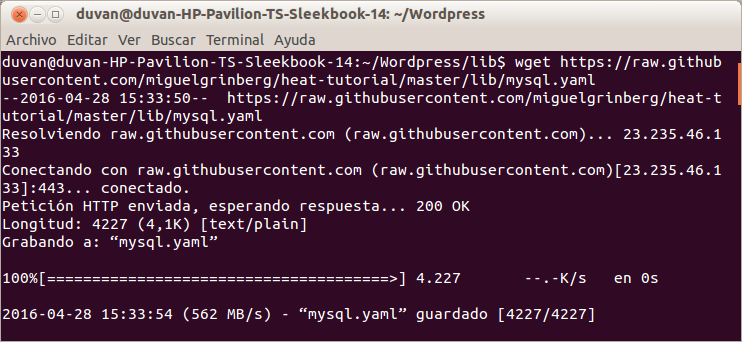
\includegraphics[scale=0.5]{11}  
	\caption{Descarga de archivos} 
\end{figure}
\newpage
\begin{figure}[ht]
	\centering
	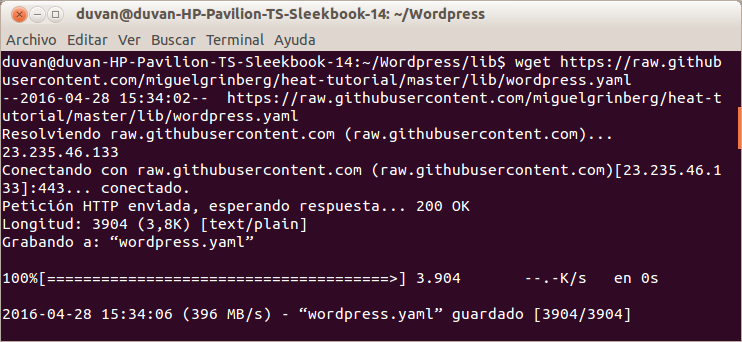
\includegraphics[scale=0.38]{12}  
	\caption{Descarga de archivos} 
\end{figure}

\begin{figure}[H]
	\centering
	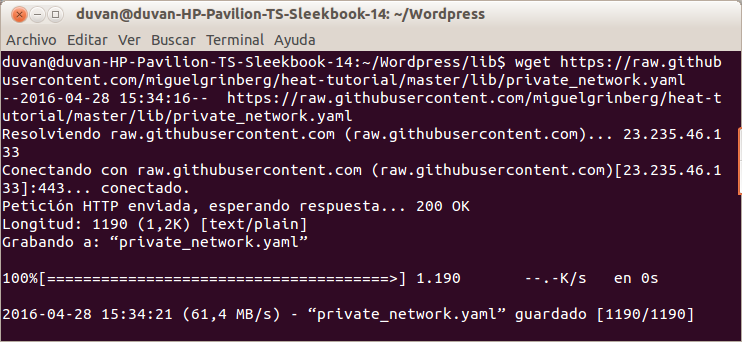
\includegraphics[scale=0.4]{13}  
	\caption{Descarga de archivos} 
\end{figure}

\begin{figure}[ht]
	\centering
	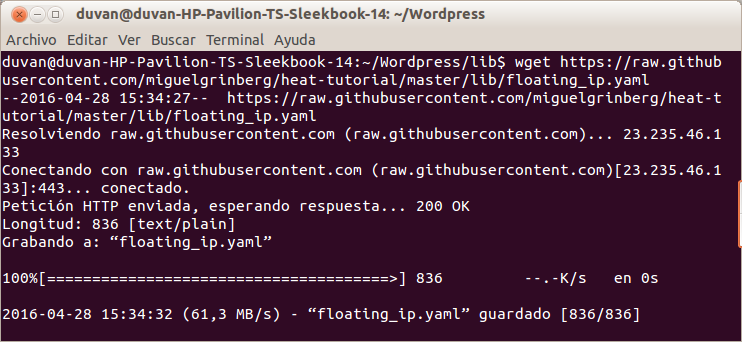
\includegraphics[scale=0.34]{14}  
	\caption{Descarga de archivos} 
\end{figure}
\newpage
\begin{figure}[ht]
	\centering
	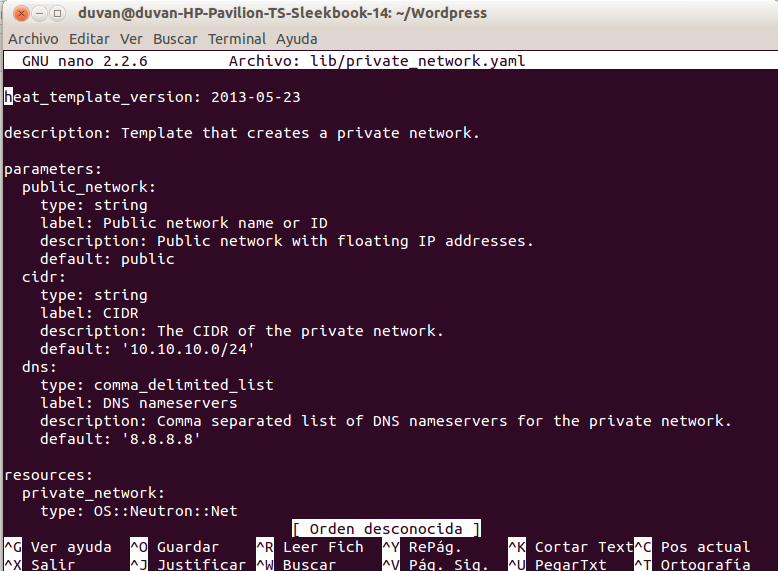
\includegraphics[scale=0.44]{15}  
	\caption{Descarga de archivos} 
\end{figure}

	
\newpage
	
	\item 	Editar el archivo  \texttt{\href{https://github.com/wilrilo/talleres/blob/master/file/taller2/wordpress-heat/lib/private_network.yaml}{lib/private\_network.yaml}} de forma que tenga el siguiente contenido.\\
	

\begin{small}
	\begin{lstlisting}[frame=single]	
heat_template_version: 2013-05-23

description: Template that creates a private network.

parameters:
public_network:
type: string
label: Public network name or ID
description: Public network with floating IP addresses.
default: public
cidr:
type: string
label: CIDR
description: The CIDR of the private network.
default: '10.10.10.0/24'
dns:
type: comma_delimited_list
label: DNS nameservers
description: Comma separated list of DNS nameservers for the private network.
default: '8.8.8.8'

resources:
private_network:
type: OS::Neutron::Net

private_subnet:
type: OS::Neutron::Subnet
properties:
network_id: { get_resource: private_network }
cidr: { get_param: cidr }
dns_nameservers: { get_param: dns }

router:
type: OS::Neutron::Router
properties:
external_gateway_info:
network: { get_param: public_network }

router-interface:
type: OS::Neutron::RouterInterface
properties:
router_id: { get_resource: router }
subnet: { get_resource: private_subnet }

outputs:
name:
description: The private network.
value: { get_attr: [private_network, name] }
	\end{lstlisting}
\end{small}

Algo interesante del enfoque planteado en este laboratorio es utilizar las plantillas previamente definidas como \textit{cajas negras}, funcionalidades ya probadas de quienes únicamente interesa sus entradas y sus salidas. Este enfoque se denomina “\textit{plantillas anidadas}” y provee una manera más extensible de depurar los diferentes despliegues orquestados.

\item Descargar el archivo \href{https://raw.githubusercontent.com/miguelgrinberg/heat-tutorial/master/heat\_3d.yaml}{heat\_3d.yaml} y se ubica en el directorio “\texttt{\href{https://github.com/wilrilo/talleres/tree/master/file/taller2/wordpress-heat}{wordpress-openstack}}”.
\newpage
\begin{figure}[ht]
	\centering
	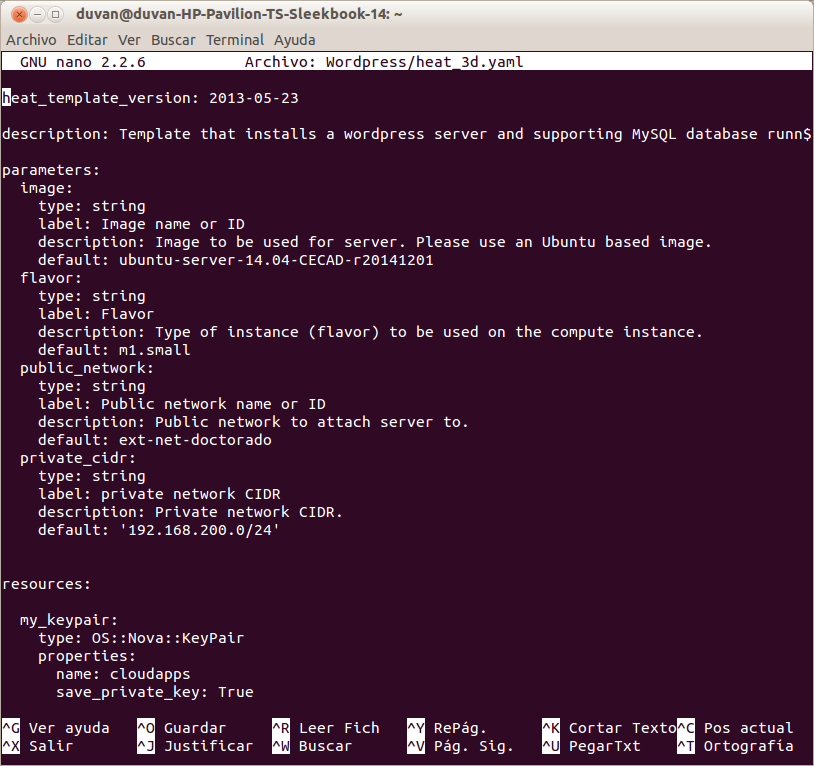
\includegraphics[scale=0.28]{heat2}  
	\caption{Descarga de archivo heat\_3d.yaml} 
\end{figure}
\item 	Realizar las modificaciones al archivo \href{https://github.com/wilrilo/talleres/blob/master/file/taller2/wordpress-heat/wordpress-deployment.yaml}{heat\_3d.yaml}, de forma que luzca como sigue a continuación:


\begin{small}
	\begin{lstlisting}[frame=single]	
heat_template_version: 2013-05-23

description: Template that installs a wordpress server and
 supporting MySQL database running on separate servers

parameters:
image:
type: string
label: Image name or ID
description: Image to be used for server. Please use an Ubuntu based image.
default: ubuntu-server-14.04-CECAD-r20141201
flavor:
type: string
label: Flavor
description: Type of instance (flavor) to be used on the compute instance.
default: m1.small
public_network:
type: string
label: Public network name or ID
description: Public network to attach server to.
default: ext-net-doctorado
private_cidr:
type: string
label: private network CIDR
description: Private network CIDR.
default: '192.168.200.0/24'


resources:

my_keypair:
type: OS::Nova::KeyPair
properties:
name: cloudapps
save_private_key: True

network:
type: Lib::CECAD::PrivateNetwork
properties:
public_network: { get_param: public_network }
cidr: {get_param: private_cidr}

mysql:
type: Lib::CECAD::MySQL
properties:
image: { get_param: image }
flavor: { get_param: flavor }
key: { get_resource: my_keypair }
private_network: { get_attr: [network, name] }
database_name: wordpress
database_user: wordpress_user

wordpress:
type: Lib::CECAD::Wordpress
properties:
image: { get_param: image }
flavor: { get_param: flavor }
key: { get_resource: my_keypair }
private_network: { get_attr: [network, name] }
mysql_server: { get_attr: [mysql, ip] }
database_name: wordpress
database_user: wordpress_user
database_password: { get_attr: [mysql, database_password] }

floating_ip:
type: Lib::CECAD::FloatingIP
properties:
port: { get_attr: [wordpress, port] }
public_network: { get_param: public_network }

outputs:
ip:
description: The public IP address to access Wordpress.
value: { get_attr: [floating_ip, ip] }
	\end{lstlisting}
\end{small}
\item 	Descargar el archivo
\href{https://raw.githubusercontent.com/miguelgrinberg/heat-tutorial/master/lib/}{env.yaml}
  en el directorio “wordpress-openstack” y editarlo teniendo en cuenta la direcciones absolutas de los archivos \href{https://github.com/wilrilo/talleres/blob/master/file/taller2/wordpress-heat/env.yaml}{*.yaml}.  

\begin{figure}[ht]
	\centering
	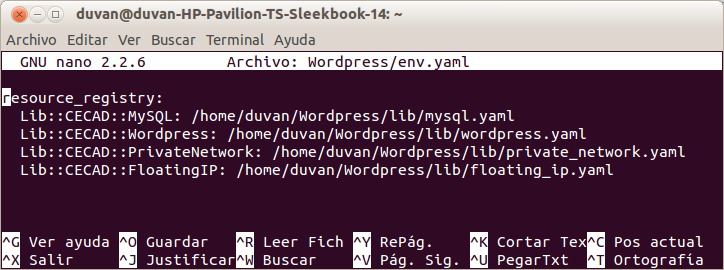
\includegraphics[scale=0.3]{env}  
	\caption{Descarga de archivo env.yaml} 
\end{figure}


\item Lanzar la pila y acceder a la consola de Wordpress en la dirección de IP flotante asignada por la orquestación. Se requiere para trabajo desde heat (en equipo en red) instalar algunos paquetes y emplear un fichero de credenciales para acceder al servidor, el fichero creds contiene lo siguiente.



\begin{figure}[H]
	\centering
	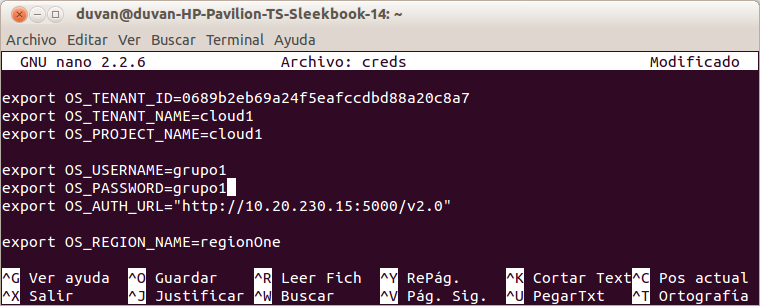
\includegraphics[scale=0.3]{creds}  
	\caption{acceso a la consola de Wordpress en la dirección de IP flotante asignada} 
\end{figure}


Por otra parte, es necesario modificar el fichero hosts e incluir algunos elementos, dependiendo de los requerimientos de cada orquestación.


\begin{figure}[H]
	\centering
	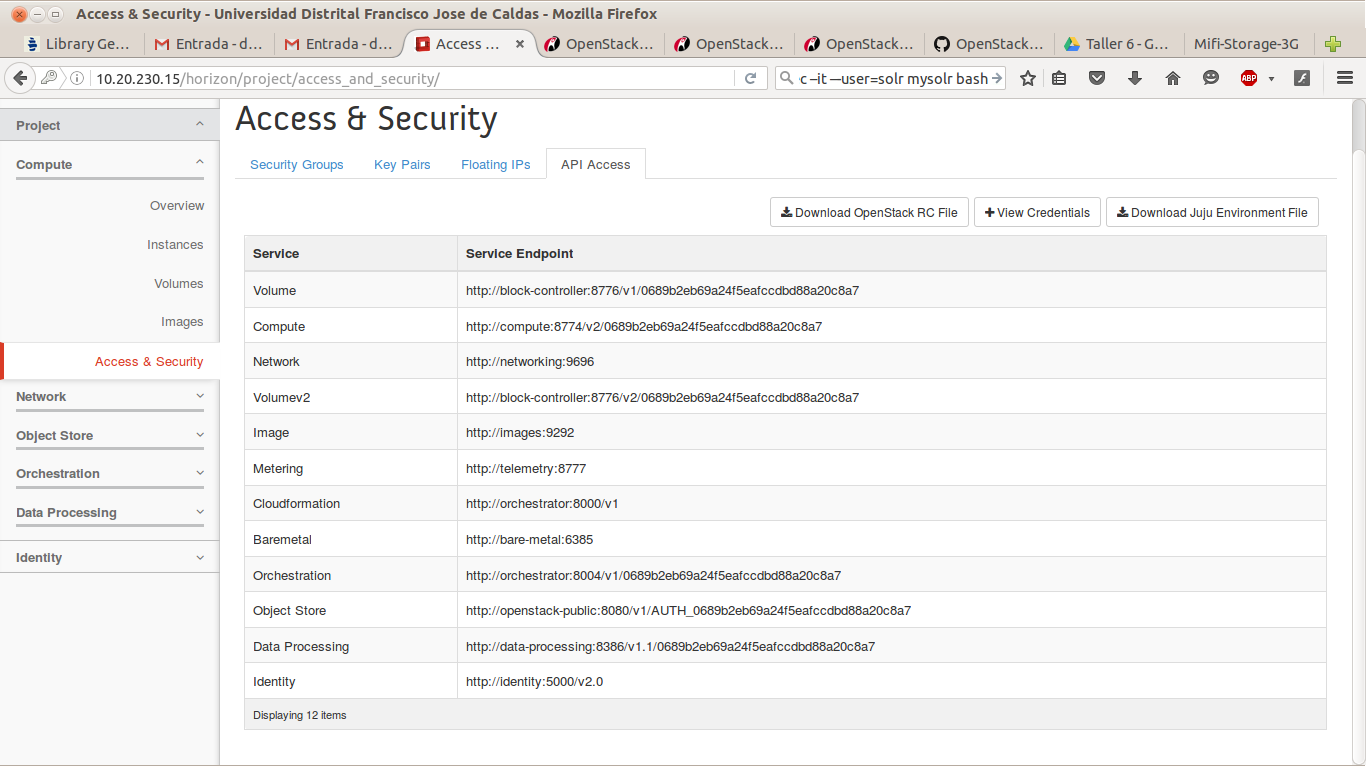
\includegraphics[scale=0.3]{AccessSecurity}  
	\caption{modificación el fichero hosts} 
\end{figure}


\begin{figure}[H]
	\centering
	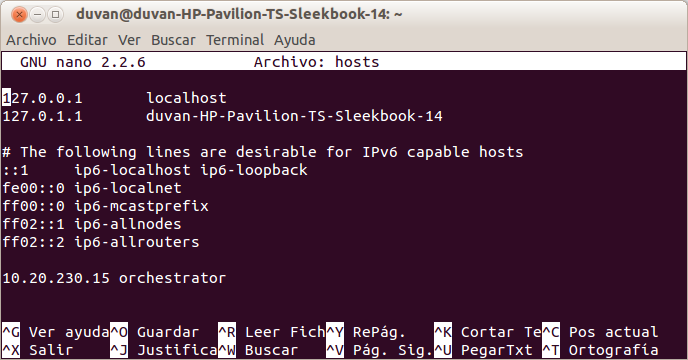
\includegraphics[scale=0.4]{hosts}  
	\caption{fichero hosts} 
\end{figure}

Para ejecutar la prueba (teniendo la carpeta creada en el directorio del usuario), se realiza el montaje de las credenciales con la función “Source”, para el ejemplo a continuación se verifica que no hay stacks en la nube:\\




\begin{figure}[ht]
	\centering
	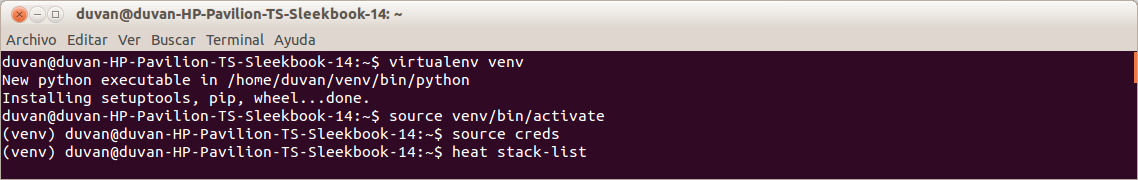
\includegraphics[scale=0.4]{espacio}  
	\caption{Espacio de trabajo y variables de entorno} 
\end{figure}
Ahora es posible lanzar la orquestación desde heat, de la siguiente manera:




\begin{figure}[ht]
	\centering
	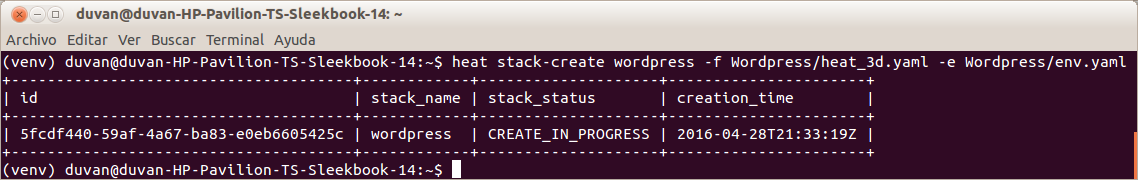
\includegraphics[scale=0.4]{orchestring}  
	\caption{Lanzamiento de la orquestación} 
\end{figure}

Por medio de la interfaz de horizon verificamos la orquestación:

\begin{figure}[H]
	\centering
	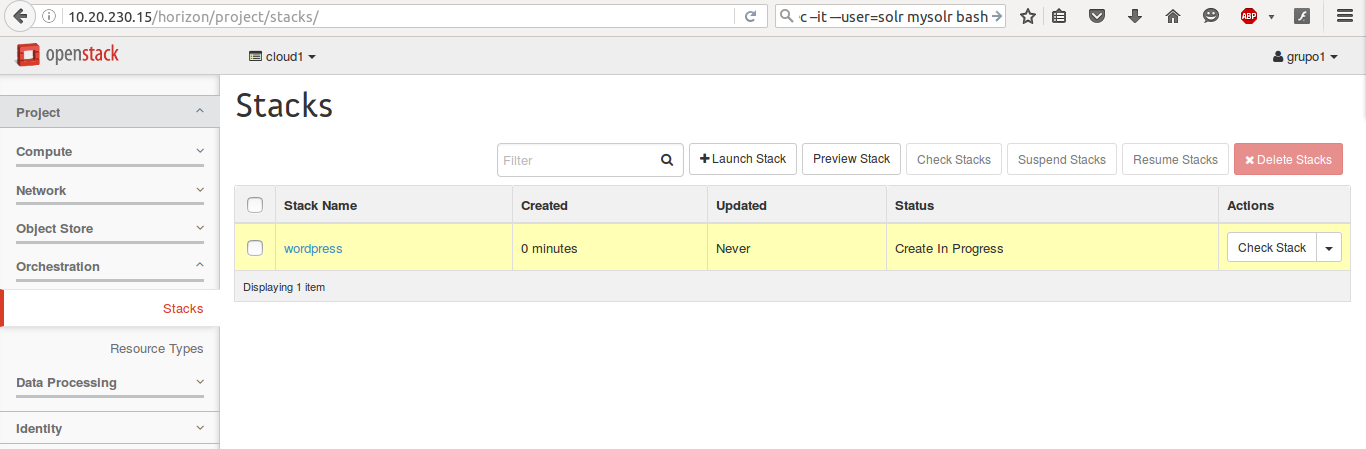
\includegraphics[scale=0.4]{Orquestando}  
	\caption{Se verifica la orquetación} 
\end{figure}


Observamos los detalles de la orquestación


\begin{figure}[ht]
	\centering
	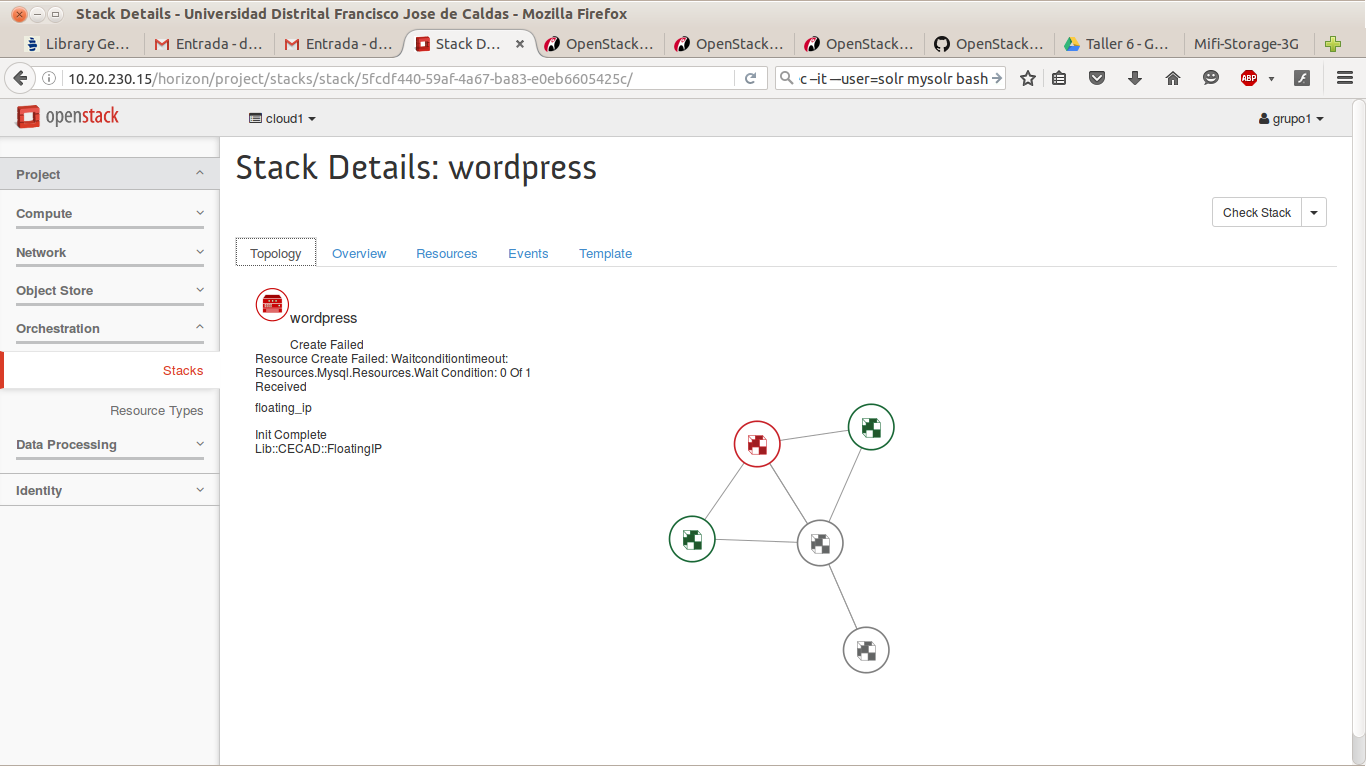
\includegraphics[scale=0.28]{Detalles}  
	\caption{Detalles de la orquestación} 
\end{figure}

\section{BIBLIOGRAFIA}
\begin{itemize}
	\item \href{http://vmartinezdelacruz.com/en-pocas-palabras-como-funciona-openstack/}{http://vmartinezdelacruz.com/en-pocas-palabras-como-funciona-openstack/}
	\item \href{https://www.openstack.org/}{https://www.openstack.org/}
	\item \href{https://www.redhat.com/es/insights/openstack}{https://www.redhat.com/es/insights/openstack}
\end{itemize}






\end{enumerate}	

\end{document}
